\documentclass[pdf]{beamer}
\usepackage[latin1]{inputenc}
\usepackage{multirow}
\usetheme{Warsaw} %Warsaw
\usecolortheme{seahorse}


\begin{document}

\title[Sequence Mapping]{Sequence Mapping/Alignment}
\subtitle{BCB 504: Applied Bioinformatics\\}
\author[Matt Settles]{Matt Settles}
\institute{University of Idaho\\ Bioinformatics and Computational Biology Program}
\date{\today}


%% Title page
\begin{frame}[plain]
  \titlepage
\end{frame}


%% Outline
\begin{frame}[plain] 
  \frametitle{Outline}
  \tableofcontents
\end{frame}

\section{Introduction}
\begin{frame}
  \frametitle{Mapping/Alignment}
Given sequence data,
\begin{description}
\item[Assembly]  seeks to put together the puzzle without knowing what the picture is 
\item[Mapping]  tries to put together the puzzle pieces directly onto an image of the picture
\end{description}
In mapping the question is more, given a small chunk of sequence, where in the genome did this piece most likely come from.
\end{frame}

\begin{frame}
\begin{center}
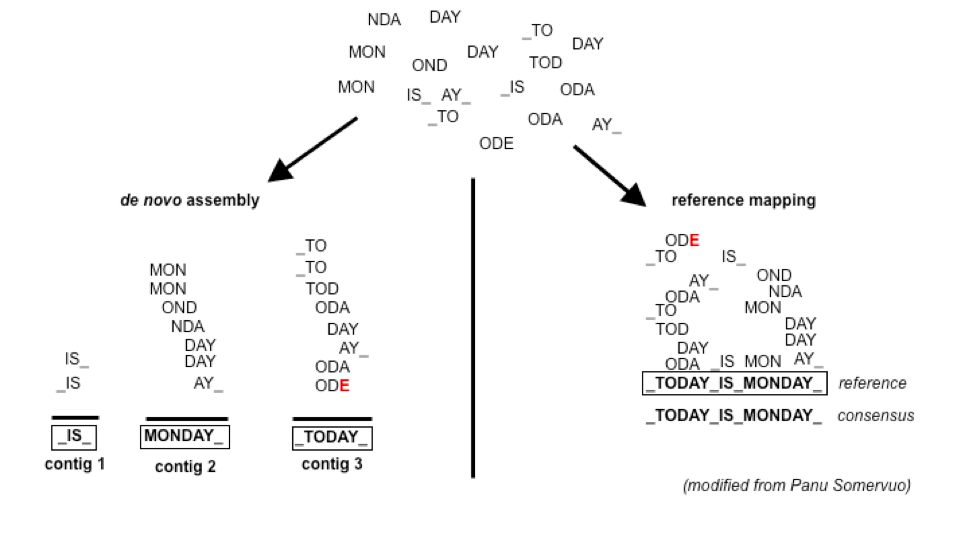
\includegraphics[scale=0.35]{Figures/Differences.png} 
\end{center}
\end{frame}

\section{Alignment Algorithms}
\subsection{BLAST}
\begin{frame}
  \frametitle{Basic Local Alignment Search Tool (BLAST)}
  Some say the first bioinformatics tool, developed at NIH and published in 1990.\\
  Problem:\\
  \begin{description}
  \item[-] Exact algorithms like Smith-Waterman and Needleman-Wunsch (dynamic programming) are slow, when the search space becomes large.
  \item[-] With the advent of automated DNA sequencing technology, the database of possible matches was becoming increasingly larger.
  \end{description}
  the BLAST algorithm emphasizes speed over sensitivity, and does not guarantee an optimal alignment.\\
  \alert{BLAST is a few to many algorithm - performs gapped alignment}
\end{frame}

\subsection{BLAT}
\begin{frame}
  \frametitle{BLAST Like Alignment Tool (BLAT)}
  Blat (Jim Kent, UCSC, 2002) was designed to solve the problem of performing comparisons between large genomes and was one of the first algorithms to efficiently search many query sequences against a large database (a genome). Blat also performs a gapped-alignment for searching RNA sequences against a genome and handling splice junctions.\\
  \begin{description}
  \item[gapped-alignment] alignment allowing for insertions and deletions greater than a few base pairs. Gapped alignment are less efficient, but more accurate.\\
  \end{description}  
  \alert{BLAT is a many to many algorithm - performs gapped alignments}
\end{frame}

\subsection{Improvements}
\begin{frame}
  \frametitle{Improving Algorithms}
  Many additional algorithms have been developed since BLAST and BLAT, mainly improving on either speed or accuracy, or both.
\end{frame}

\section{Illumina Data}
\begin{frame}
and then came Illumina data -\\
New Problem:\\
\begin{itemize}
\item We still have a large search space (aka genome)
\item Very small pieces, many possible close matches
\item Millions or tens of millions of query sequences
\end{itemize}
\end{frame}

\begin{frame}
  \frametitle{Types}
  \begin{description}
  \item[Hash based] First generation of alignment algorithms relied on hashes (Eland [Illumina], RMAP, MAQ, SHRiMP, SOAP)
  \item [Burrows-Wheeler] Second generation algorithms with a reduced memory footprint (BWA, SOAP2, Bowtie)
  \end{description}
\end{frame}

\begin{frame}
\begin{center}
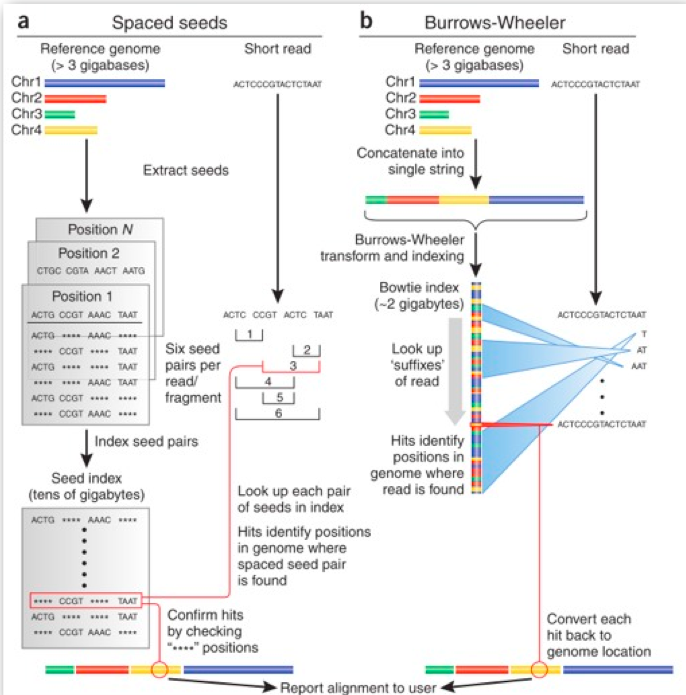
\includegraphics[scale=.32]{Figures/hashVsBW.png} 
\end{center}
\end{frame}

\subsection{Hash Based}
\begin{frame}
  \frametitle{hash based example: MAQ}
  \begin{itemize}
  \item  Index reference genome (or sequence reads) $=>$ creates hash index       
  \begin{itemize}
   \item Big file: $>$50GB 
   \item takes a long time (hours or overnight), but only need to do once
  \end{itemize}
  \item Divide each read into segments (seeds) and look up in table
  \begin{itemize}
  \item Search stage finds regions in the genome that can potentially be homologous to the read. 
  \item Alignment stage verifies these regions to check if they are indeed homologous. More computationally intensive
  \end{itemize}
  \end{itemize}
\end{frame}

\subsection{Burrows-Wheeler Tranform}
\begin{frame}
  \frametitle{burrows-wheeler example: Bowtie2}
   Used in data compression (e.g. bzip) $=>$ index: much smaller than hash-based index ($<$2GB)
\begin{itemize}
\item Alignment speed: 30x faster than MAQ
\end{itemize}
Steps:\\
\begin{itemize}
\item Create BWT index of genome
\item Align read 1 character at a time to BWT-transformed genome
\end{itemize}
\end{frame}

\begin{frame}
\begin{center}
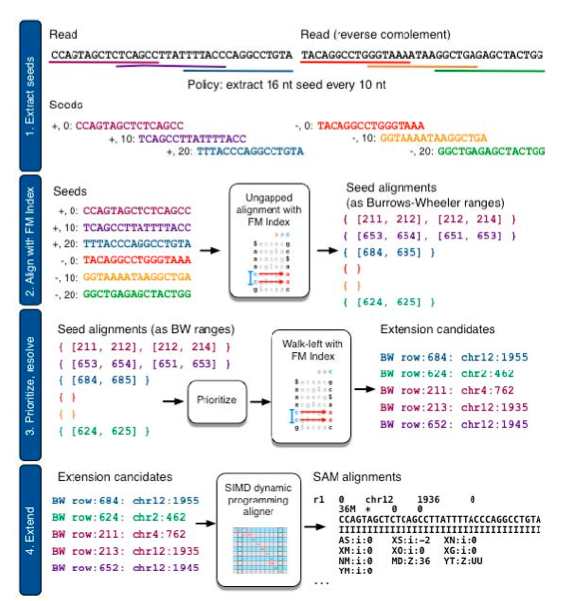
\includegraphics[scale=.35]{Figures/BWT.png} 
\end{center}
\end{frame}

\begin{frame}
\frametitle{considerations}
\begin{itemize}
\item placing reads in regions that do not exist in the reference genome
\item sequencing errors and variations: alignment between read and true source in genome may have more differences than alignment with some other copy of repeat.
\item What if many nucleotide differences with closest fully sequenced genome? (3\% is a common alignment capability)
\item placing reads in repetitive regions: Some algorithms only return 1 mapping; If multiple: map quality = 0
\item algorithms that use paired-end information $=>$ might prefer correct distance over correct alignment.
\end{itemize}
\end{frame}

\section{SAM/BAM output}
\begin{frame}
\frametitle{SAM/BAM format}
\begin{description}
\item [SAM] (Sequence Alignment/Map) format = unified format for storing read alignments to a reference genome
\item [BAM] = binary version of SAM for fast querying
\end{description}
\end{frame}

\begin{frame}
\begin{center}
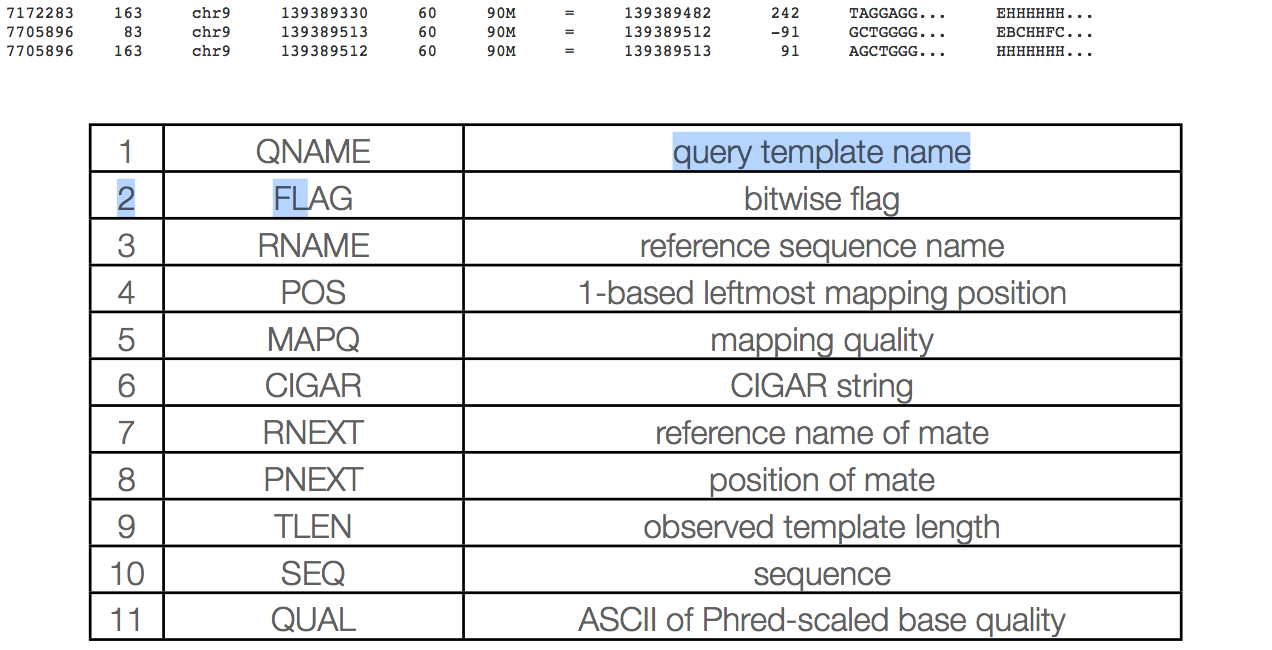
\includegraphics[scale=0.25]{Figures/sam.png} 
\end{center}
\end{frame}
\end{document}
